\chapter{Mozaik}
\section{Práce s frameworkem}

Mozaik je framework pro Python, pomocí kterého lze snadno specifikovat 2-rozměrné vrstvy neuronů, nad kterými pak běží experimenty. Experimenty produkují data, která lze analyzovat různými algoritmy a~zaznamenávat jejich výstupy. V Mozaik tutorialu\footnote{\url{https://github.com/CSNG-MFF/mozaik/blob/master/doc/source/tutorial.1.rst}} je ukázán příklad, na který se zde (v~trochu zkrácené podobě) podíváme.

\begin{figure}
  \centering
  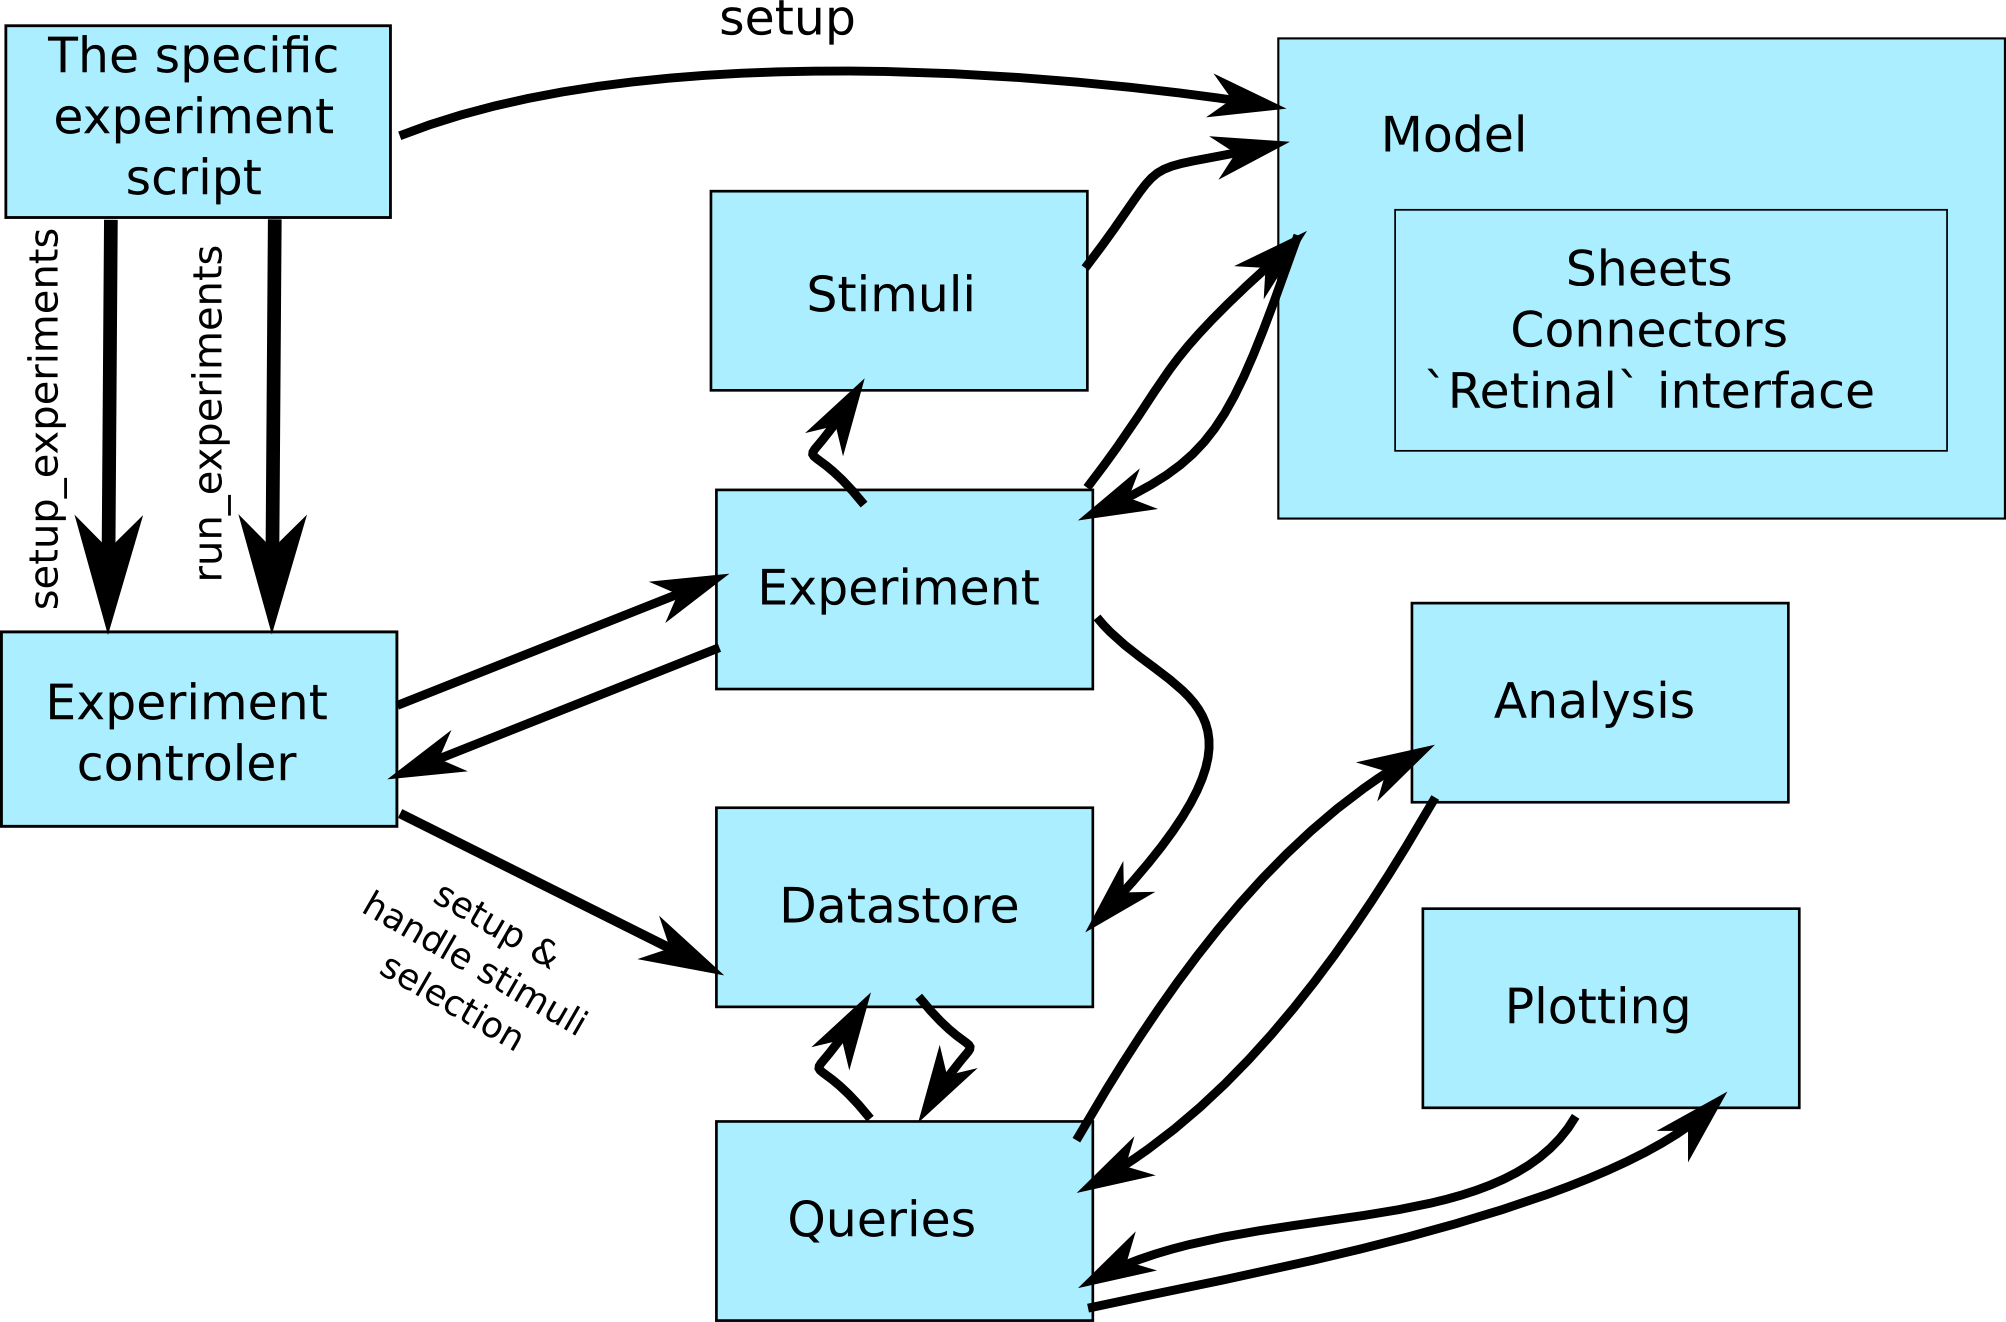
\includegraphics[width=.6\linewidth]{img/mozaik_control_flow.png}
  \caption{Control flow mezi jednotlivými komponentami Mozaiku\cite{MozaikIntroduction}}
\end{figure}

Kód je rozdělen na 6~hlavních částí. Část 1 a~2 jsou definice neuronových vrstev - třída \lstinline|Model| a~její parametry:

\begin{lstlisting}[language=Python]
  class VogelsAbbott( Model ):
    # parametry jsou nacteny z oddeleneho souboru
    required_parameters = ParameterSet({
      # definujeme 2 neuronove vrstvy
      'sheets': ParameterSet({
          'exc_layer': ParameterSet,
          'inh_layer': ParameterSet, 
      })
    })

    def __init__(self, sim, num_threads, parameters):
      Model.__init__(self, sim, num_threads, parameters)
      # nacteni komponent vrstev
      ExcLayer = load_component(
        self.parameters.sheets.exc_layer.component
      )
      ...
      
      exc = ExcLayer(
        self, 
        self.parameters.sheets.exc_layer.params
      )
      ...

      # spojeni mezi vrstvami
      UniformProbabilisticArborization(
        self,'ExcExcConnection',exc,exc,
        self.parameters.sheets.exc_layer.ExcExcConnection
      ).connect()
      ...
\end{lstlisting}

Dále je potřeba specifikovat samotné experimenty, které chceme na mozku provést.

\begin{lstlisting}[language=Python]
def create_experiments(model):
  return [
    #Lets kick the network up into activation
    PoissonNetworkKick(model,ParameterSet({
      'duration': 8*7,
      'drive_period': 8*7.0,
      'sheet_list': ["Exc_Layer","Inh_Layer"],
      'stimulation_configuration' : {
        'component':
          'mozaik.sheets.population_selector'
          '.RCRandomPercentage',
        'params': {'percentage' : 20.0}
      },
      'lambda_list': [100.0,100.0],
      'weight_list': [0.1,0.1]
    })),
    #Spontaneous Activity 
    NoStimulation(model,ParameterSet({'duration': 135.0*2}))
  ]
\end{lstlisting}

Experimenty produkují surová data, \emph{segmenty}. Ta nám sama o sobě moc neřeknou, ale můžeme na nich spouštět analytické algoritmy. Ještě předtím ale spustíme samotnou simulaci.

\begin{lstlisting}[language=Python]
data_store,model = run_workflow(
  'example simulation',
  VogelsAbbott,
  create_experiments
)
\end{lstlisting}

Segmenty jsou uložené v datastore a nám už nic nebrání je analyzovat.

\begin{lstlisting}[language=Python]
def perform_analysis_and_visualization(data_store):
  analog_ids = sorted(
    param_filter_query(data_store,sheet_name="Exc_Layer") \
    .get_segments()[0].get_stored_esyn_ids()
  )
  ...

  
  PopulationMeanAndVar(
    data_store,ParameterSet({'ignore_nan_and_inf': False})
  ).analyse()
  ...
\end{lstlisting}

V tuto chvíli můžeme použít modul \lstinline|mozaik.visualization| a vygenerovat množství rozmanitých grafů, které se uloží jako png soubory. My ale tuto funkcionalitu používat nebudeme a podíváme se raději na různé typy datových struktur, které se v datastore mohou nacházet.

\section{Datastore}

Datastore se na disk serializuje ve formátu pickle, což je binární protokol pro serializaci python objektů. Kromě \emph{ADS}~(analysis data structure) se v něm nachází metadata o neuronech, jejich vrstvách a stimulech. ADS lze vyhledávat pomocí jejich parametrů. ADS může být (ale nemusí) být spojena s konkrétní vrstvou, stimulem, nebo konkrétním neuronem. Dělí se na několik typů, podle typu dat, které uchovávají.

\subsection{SingleValue}

V celku triviální wrapper pro jedinou hodnotu.

\subsection{SingleValueList}

Jednorozměrný seznam hodnot.

\subsection{PerNeuronValue}

Podobná datová struktura jako SingleValueList, ale každá hodnota v seznamu odpovídá konkrétnímu neuronu.

\subsection{PerNeuronPairValue}

Seznam neuronů a matice hodnot pro každý jejich pár.

\subsection{AnalogSignal}

Jde o wrapper nad Neo \lstinline|AnalogSignal| \footnote{\url{https://neo.readthedocs.io/en/stable/api_reference.html\#neo.core.AnalogSignal}}, což je dvourozměrné pole periodicky měřených hodnot. Jedna dimenze odpovídá času a druhá jednotlivým zaznamenávaným kanálům. V praxi se ale v Mozaiku do AnalogSignalu zaznamenává pouze jeden kanál, takže se hodí o něm uvažovat jako o jednorozměrném poli.

\subsection{AnalogSignalList}

Kombinace PerNeuronValue a AnalogSignal. Seznam AnalogSignalů, kde každý AnalogSignal náleží specifickému neuronu.

\subsection{PerNeuronPairAnalogSignalList}

Tentokrát jde o kombinaci AnalogSignalu a PerNeuronPairValue. Seznam neuronů a matice AnalogSignalů pro každý jejich pár.

\subsection{ConductanceSignalList}

Jedná se o rozšířený AnalogSignalList s tím, že pro každý neuron jsou zde uloženy 2 AnalogSignaly.

\subsection{Connections}

Tato datová struktura popisuje spojení mezi neurony, což jsou orientované hrany v grafu. Každá hrana má navíc ještě specifikovanou váhu a zpoždění.

\section{Předchozí práce}

Tato práce navazuje na ročníkový projekt Kateřiny Čížkové~\cite{Cizkova2020nprg035}. Její program byla webová aplikace, která umožňovala interaktivně zobrazit neuronové vrstvy v~zadaném datastore. Původní záměr byl tento projekt rozšířit, ale, jak je v~dokumentaci projektu popsáno, kolegyně zvolila ne úplně vhodnou technologii a~doporučuje začít potenciálně zcela od začátku. Tato práce tedy namísto Python frameworku Bokeh používá Flask a~renderování vizualizací je specifikováno až ve frontendu (více podrobností je v~kapitole XX). Podobnost kódu je naprosto minimální, nicméně zejména ze začátku sloužil jako výborná inspirace.